\documentclass[12pt,a4paper]{article}
\usepackage[utf8x]{inputenc}
%\usepackage{ucs}
\usepackage[french]{babel}
\usepackage[T1]{fontenc}
\usepackage{amsmath}
\usepackage{amsfonts}
\usepackage{amssymb}
	\everymath{\displaystyle}
\usepackage[table]{xcolor}
\usepackage{graphicx}
	\setkeys{Gin}{width=0.7071\linewidth}
\usepackage{lmodern}
\usepackage[left=2cm,right=2cm,top=2cm,bottom=2cm]{geometry}
\author{ F.L.G.}
\title{Modèle du cours cycle 5}
\usepackage{array}
	\renewcommand{\arraystretch}{1.25}
\usepackage{multirow}
\usepackage{multicol}
\setlength{\columnseprule}{1pt}
\usepackage{float}
	\floatplacement{table}{H}
	\floatplacement{figure}{H}
\usepackage{tikz}
	\usetikzlibrary{math, babel, patterns}
\usepackage[tikz]{bclogo}
%\usepackage{siunitx}
%	\sisetup{
%		locale=FR,
%	} %end sisetup
\usepackage{hyperref}
\hypersetup{
	colorlinks=true,
	linkcolor=cyan,
	urlcolor=blue,
	filecolor=pink}
\urlstyle{same}
\usepackage{pgfplots}
\usepackage{ifthen}
	\newboolean{isEvaluated}
	\setboolean{isEvaluated}{False}
	\newboolean{isCorrection}
	\setboolean{isCorrection}{False}

\renewcommand{\thesection}{$\looparrowright$\Roman{section}}
\begin{document}
%%% CARTOUCHE D'IDENTIFICATION %%%
\begin{flushleft}
\begin{tabular}{| m{0.15\linewidth} m{0.78\linewidth} |}
	\hline
	\multirow{4}{*}{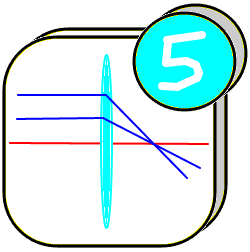
\includegraphics[width=\linewidth]{cycle5-logo-optique.png}}	
	& c5-1.pX.acY
	\begin{LARGE}
	Les lois de réfraction et de réflexion
	\end{LARGE} \\ [0.5ex]
	\cline{2-2}
	 & \cr
	 & NOM : . \ . \ . \ . \ . \ . \ . \ . \ . \ . \ . Prénom : . \ . \ . \ . \ . \ . \ . \ . \ . \ . \ . \\
	 & \cr
	 & Classe : . \ . \ . \ . Durée : 80 min. \\ [1ex]
	\hline
\end{tabular}

%%% CARTOUCHE DE NOTATION %%%
\ifthenelse{\boolean{isEvaluated}}{%true
	\begin{tabular}{| m{0.18\linewidth} | m{0.7575\linewidth} |}
		\hline
		Note : & Appréciation \\
		 & \\
		 & \\
		 & \\
		 & \\
		\hline
	\end{tabular}
}{%false
\relax
}%fin

%%% CARTOUCHE D'ÉVALUATION DES COMPÉTENCES %%%
\begin{tabular}{| m{0.05\linewidth} | m{0.725\linewidth} | m{0.015\linewidth} | m{0.015\linewidth} | m{0.015\linewidth} | m{0.015\linewidth} |}
\hline
\multirow{2}{*}{Réf.} & \multirow{2}{*}{Intitulé Compétences cycle 5} & \multicolumn{4}{c |}{État} \\
\cline{3-6}
	& & I & F & S & T \\
\hline
%Ap 1 & Énoncer une problématique. & & & & \\ \hline
%Ap 2 & Rechercher et organiser l’information en lien avec la problématique étudiée. & & & & \\ \hline
%Ap 3 & Représenter la situation par un schéma. & & & & \\ \hline
Ra 1 & Formuler des hypothèses. & & & & \\ \hline
Ra 2 & Proposer une stratégie de résolution. & & & & \\ \hline
%Ra 3 & Planifier des tâches. & & & & \\ \hline
%Ra 4 & Évaluer des ordres de grandeur. & & & & \\ \hline
%Ra 5 & Choisir un modèle ou des lois pertinentes. & & & & \\ \hline
Ra 6 & Choisir, élaborer, justifier un protocole. & & & & \\ \hline
%Ra 7 & Faire des prévisions à l'aide d'un modèle. & & & & \\ \hline
%Ra 8 & Procéder à des analogies. & & & & \\ \hline
%Ré 1 & Mettre en œuvre les étapes d’une démarche. & & & & \\ \hline
Ré 2 & Utiliser un modèle. & & & & \\ \hline
Ré 3 & Effectuer des procédures courantes (calculs, représentations, collectes de données, etc.). & & & & \\ \hline
%Ré 4 & Mettre en \oe{}uvre un protocole expérimental en respectant les règles de sécurité. & & & & \\ \hline
%Va 1 & Faire preuve d’esprit critique, procéder à des tests de vraisemblance. & & & & \\ \hline
%Va 2 & Identifier des sources d’erreur, estimer une incertitude, comparer à une valeur de référence. & & & & \\ \hline
Va 3 & Confronter un modèle à des résultats expérimentaux. & & & & \\ \hline
%Va 4 & Proposer d’éventuelles améliorations de la démarche ou du modèle. & & & & \\ \hline
%Co 1 & présenter une démarche de manière argumentée, synthétique et cohérente. & & & & \\ \hline
%Co 2 & utiliser un vocabulaire adapté et choisir des modes de représentation appropriés & & & & \\ \hline
%Co 3 & échanger entre pairs. & & & & \\ \hline
\end{tabular}

\end{flushleft}
%%%%% DÉBUT DU COURS %%%%%
\section{Un crayon magique ?}
\begin{figure}
	\centering
	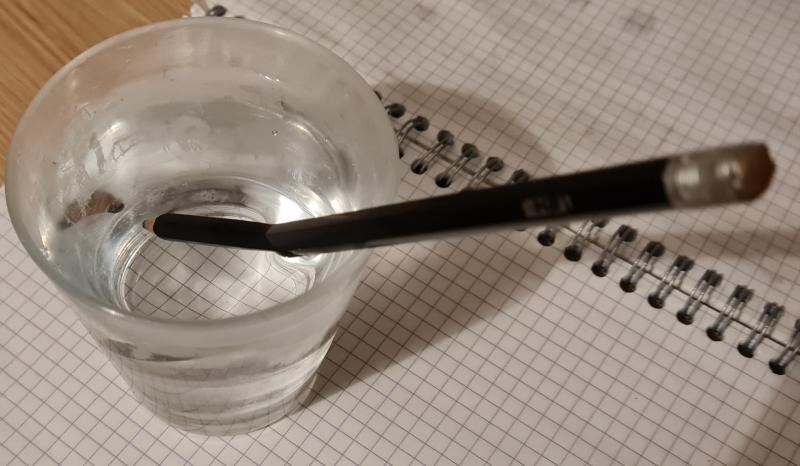
\includegraphics{crayon-magique.jpg}
\end{figure}
\paragraph*{Situation.}
Les méthodes traditionnelle de pêche dans de nombreuses peuplades indigène --ou quelques aventuriers de séries télévisées-- utilisent des lances pour harponner des poissons. 
Les amateurs sont confrontés à un problème de taille : suivant l'angle du soleil, le poisson évite le harpon, la trajectoire semble bonne pourtant vu par l'humain.

La situation est symbolisée dans l'image précédente qui montre un crayon à papier plongé partiellement dans un verre d'eau.

\paragraph*{Votre travail.}
Il consiste à proposer une expérience permettant d'établir la relation qui peut exister entre l'angle que forme le crayon avec la surface et celui du même crayon dans l'eau.

Comme d'habitude sont attendus~:
\begin{itemize}
	\item une liste du matériel (fournie exceptionnellement)
	\item un ou plusieurs schémas légendés
	\item un protocole indiquant les informations à mesurer.
\end{itemize}

\paragraph*{Matériel à disposition.}
Sur la paillasse du professeur se trouve le matériel qui peut être utilisé, à vous d'opter pour celui qui vous semble pertinent.

\begin{figure}
	\centering
	\begin{tikzpicture}
		\draw[dotted, step=0.5cm, ultra thin](0,0) grid (\linewidth,22) ;
	\end{tikzpicture}
\end{figure}
\newpage
\section{Étude expérimentale simulée.}
\begin{multicols}{2}
	\begin{figure}
		\centering
		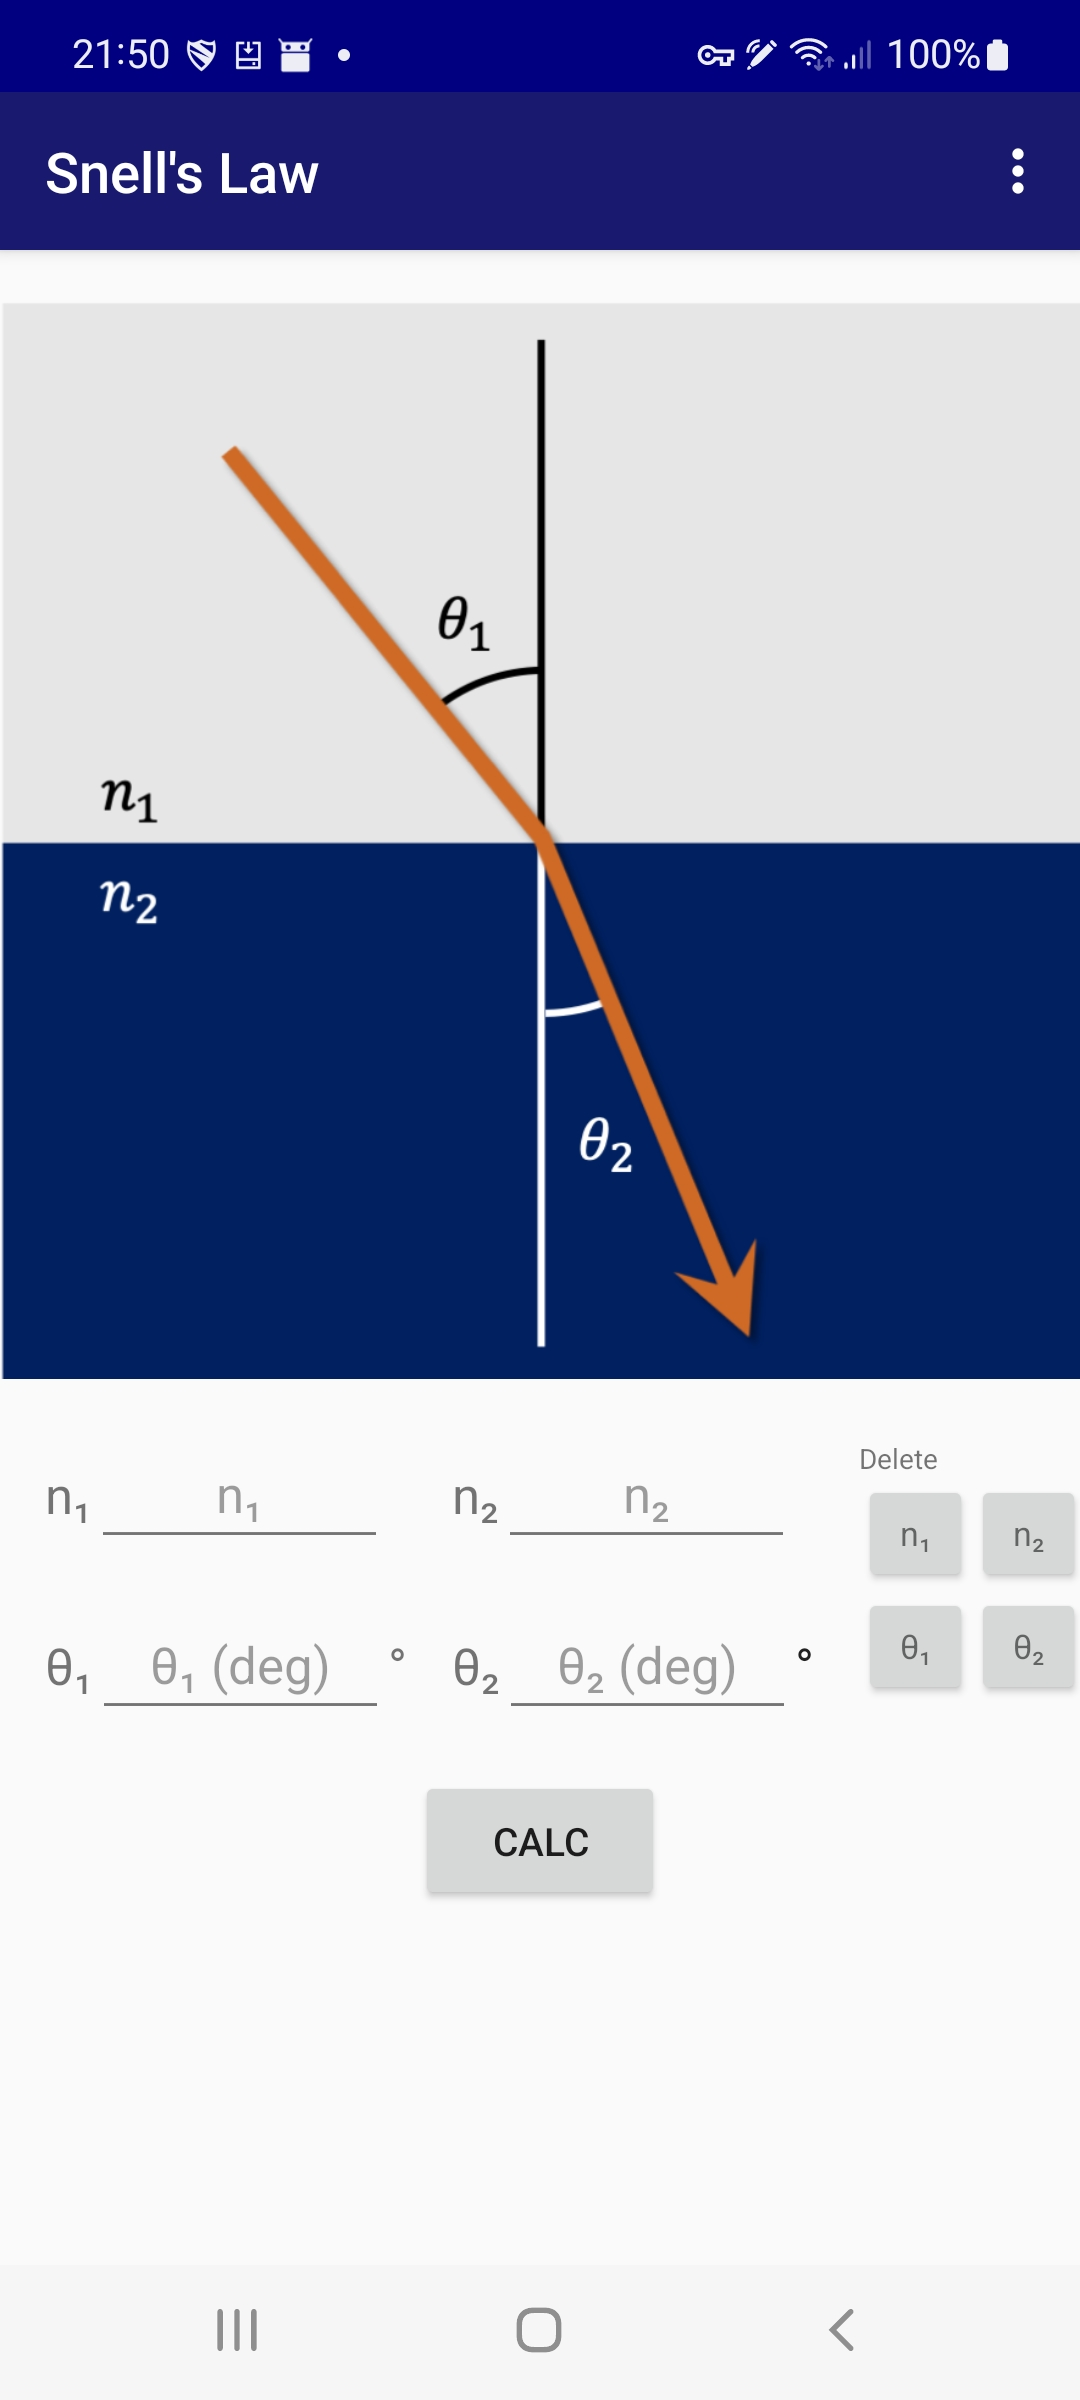
\includegraphics{Snell_s-Law.jpg}
	\end{figure}
\columnbreak

\paragraph{Matériel.}\hfill

Sur vos paillasse se trouve un \emph{smartphone}, exécutez l'application \emph{Snell's Law}.

\vspace{2cm}

Saisissez les incides des milieux transparents 1 et 2, puis l'angle $\theta_1$ et appuyez sur le bouton \boxed{Calc}. 

\vspace{2cm}

Pour effectuer ensuite un calcul, pensez à utiliser les boutons à droite pour effacer les valeurs d'angle $\theta_1$ et $\theta_2$.

\vspace{15mm}

Complétez le tableau qui suit
\end{multicols}
\paragraph*{Tableau des} données expérimentales simulées.
\begin{table}
	\centering
	\begin{tabular}{c | c | c | c | c | c | c | c | c | c | c | c | c | c | c | c | c | c | c | c}
		$\theta_1$ & 0 & 5 & 10 & 15 & 20 & 25 & 30 & 35 & 40 & 45 & 50 & 55 & 60 & 65 & 70 & 75 & 80 & 85 \cr
		\hline
		$\theta_2$ & & & & & & & & & & & & & & & & & & \cr
	\end{tabular}
\end{table}
\vspace{2cm}

\paragraph{Question.} Y a-t-il relation de proportionnalité entre $\theta_1$ et $\theta_2$~? Expliquez votre réponse en vous appuyant sur les données expérimentales. \newline
\noindent . \ \ . \ \ . \ \ . \ \ . \ \ . \ \ . \ \ . \ \ . \ \ . \ \ . \ \ . \ \ . \ \ . \ \ . \ \ . \ \ . \ \ . \ \ . \ \ . \ \ . \ \ . \ \ . \ \ . \ \ . \ \ . \ \ . \ \ . \ \ . \ \ . \ \ . \ \ . \ \ . \ \ . \ \ . \ \ . \ \ . \ \ . \ \ . \ \ . \ \ . \ \ . \ \ . \ \ . \ \ . \ \ . \ \ . \ \ . \ \ . \ \ . \ \ . \ \ . \ \ . \ \ . \ \ . \ \ . \ \ . \ \ . \ \ . \ \ . \ \ . \ \ . \ \ . \ \ . \ \ . \ \ . \ \ . \ \ . \ \ . \ \ . \ \ . \ \ . \ \ . \ \ . \ \ . \ \ . \ \ . \ \ . \ \ . \ \ . \ \ . \ \ . \ \ . \ \ . \ \ . \ \ . \ \ . \ \ . \ \ . \ \ . \ \ . \ \ . \ \ . \ \ . \ \ . \ \ . \ \ . \ \ . \ \ . \ \ . \ \ . \ \ . \ \ . \ \ . \ \ . \ \ . \ \ . \ \ . \ \ . \ \ . \ \ . \ \ . \ \ . \ \ . \ \ . \ \ . \ \ . \ \ . \ \ . \ \ . \ \ . \ \ . \ \ . \ \ . \ \ . \ \ . \ \ . \ \ . \ \ . \ \ . \ \ . \ \ . \ \ . \ \ . \ \ . \ \ . \ \ . \ \ . \ \ . \ \ . \ \ . \ \ . \ \ . \ \ . \ \ . \ \ . \ \ . \ \ . \ \ . \ \ . \ \ . \ \ . \ \ . \ \ . \ \ . \ \ . \ \ . \ \ . \ \ . \ \ . \ \ . \ \ . \ \ . \ \ . \ \ . \ \ . \ \ . \ \ . \ \ . \ \ . \ \ . \ \ . \ \ . \ \ .
\newpage
\section{Étude expérimentale classique : étude de la réflexion.}
\paragraph*{Matériel.}
Vous disposez sur votre paillasse en plus du \emph{smartphone} d'un miroir miniature, d'un laser monochromatique et d'un rapporteur.

\paragraph*{Consigne.}
Mesurez l'angle d'incidence $\theta_i$ avec lequel un rayon venant du laser et frappant le miroir et celui de l'angle rebondi $\theta_r$. Complétez le schéma et le tableau qui suivent.

\paragraph*{Schéma.} Dans le cadre ci-dessous, schématisez l'expérience réalisée, inspirez-vous du schéma du paragraphe précédent.
\begin{figure}
	\centering
	\begin{tikzpicture}
		\draw[dashed, black!50!white](0,0) rectangle (\linewidth,8) ;
		\ifthenelse{\boolean{isCorrection}}{%true
			\draw[dashed, red](0,4) -- ++(0.70\linewidth,0) ;
			\draw[pattern=north east lines] (3,0.5) node[above left]{Miroir} rectangle ++(1,7) ;
			\draw[->, blue, line width=1.5] (10,6.5) -- (7,5.25) node[below right] {Rayon incident} ;
			\draw[->, blue, line width=1.5] (7,5.25) -- (4,4) ;
			\draw[->, red!50!blue, line width=1.5] (4,4) -- (7,2.75) ;
			\draw[->, red!50!blue, line width=1.5] (7,2.75) -- (10,1.5) node[right] {Rayon réfléchi} ;
			\draw[->, blue] (5,4) arc (0:20:1) node[right] {~~$\theta_i$} ;
			\draw[->, red!50!blue] (5.5,4) arc (0:-20:1.5) node[right] {~~$\theta_r$} ;
			\draw[rotate around={22:(4,4)}, fill=white!90!blue] (10.5,3.5) node[below right] {Laser} rectangle ++(3,1) ;
		}{
		\node at (0,0) {} ;		
		};%end
	\end{tikzpicture}
\end{figure}

\paragraph{Données expérimentales.} Complétez le tableau
\begin{table}
	\centering
	\renewcommand*{\arraystretch}{1.25}
	\rowcolors{1}{white!90!black}{white}
	\begin{tabular}{m{0.1\linewidth} | m{0.1\linewidth} | m{0.1\linewidth} | m{0.1\linewidth} | m{0.1\linewidth} | m{0.1\linewidth} | m{0.1\linewidth} |}
		$\theta_i$ & 0 & 15 & 30 & 45 & 60 & 75 \cr
		\hline
		$\theta_r$ & & & & & & \cr
	\end{tabular}
\end{table}
\paragraph{Conclusion.} En vous appuyant sur vos résultats expérimentaux, trouvez une relation entre les deux angles.

\noindent . \ \ . \ \ . \ \ . \ \ . \ \ . \ \ . \ \ . \ \ . \ \ . \ \ . \ \ . \ \ . \ \ . \ \ . \ \ . \ \ . \ \ . \ \ . \ \ . \ \ . \ \ . \ \ . \ \ . \ \ . \ \ . \ \ . \ \ . \ \ . \ \ . \ \ . \ \ . \ \ . \ \ . \ \ . \ \ . \ \ . \ \ . \ \ . \ \ . \ \ . \ \ . \ \ . \ \ . \ \ . \ \ . \ \ . \ \ . \ \ . \ \ . \ \ . \ \ . \ \ . \ \ . \ \ . \ \ . \ \ . \ \ . \ \ . \ \ . \ \ . \ \ . \ \ . \ \ . \ \ . \ \ . \ \ . \ \ . \ \ . \ \ . \ \ . \ \ . \ \ . \ \ . \ \ . \ \ . \ \ . \ \ . \ \ . \ \ . \ \ .


\newpage
\section{Un peu de cours : La loi de \bsc{Snell-Descartes} sur la réflexion et la réfraction.}

\subsection{Réflexion.}
\begin{bclogo}[nobreak=true, couleur=red!5, logo=\bccoeur, arrondi=0.1]{À Retenir}
\ifthenelse{\boolean{isCorrection}}{%true
{\color{red}{\large{%
Lorsqu'un rayon lumineux traverse un milieu transparent  avec un angle d'incidence $i_1$ par rapport à la normale d'une surface réfléchissante, il repart avec un angle $i_R$ par rapport à cette normale tels que~:
$$
	i_R = i_1
$$
}}}
}{%false
\noindent . \ \ . \ \ . \ \ . \ \ . \ \ . \ \ . \ \ . \ \ . \ \ . \ \ . \ \ . \ \ . \ \ . \ \ . \ \ . \ \ . \ \ . \ \ . \ \ . \ \ . \ \ . \ \ . \ \ . \ \ . \ \ . \ \ . \ \ . \ \ . \ \ . \ \ . \ \ . \ \ . \ \ . \ \ . \ \ . \ \ . \ \ . \ \ . \ \ . \ \ . \ \ . \ \ . \ \ . \ \ . \ \ . \ \ . \ \ . \ \ . \ \ . \ \ . \ \ . \ \ . \ \ . \ \ . \ \ . \ \ . \ \ . \ \ . \ \ . \ \ . \ \ . \ \ . \ \ . \ \ . \ \ . \ \ . \ \ . \ \ . \ \ . \ \ . \ \ . \ \ . \ \ . \ \ . \ \ . \ \ . \ \ . \ \ . \ \ . \ \ . \ \ . \ \ . \ \ . \ \ . \ \ . \ \ . \ \ . \ \ . \ \ . \ \ . \ \ . \ \ . \ \ . \ \ . \ \ . \ \ . \ \ . \ \ . \ \ . \ \ . \ \ . \ \ . \ \ . \ \ . \ \ . \ \ . \ \ . \ \ . \ \ . \ \ . \ \ . \ \ . \ \ . \ \ . \ \ . \ \ . \ \ . \ \ . \ \ . \ \ . \ \ . \ \ . \ \ . \ \ . \ \ . \ \ . \ \ . \ \ . \ \ . \ \ . \ \ . \ \ . \ \ . \ \ . \ \ . \ \ . \ \ . \ \ . \ \ . \ \ . \ \ . \ \ . \ \ . \ \ . \ \ . \ \ . \ \ . \ \ . \ \ . \ \ . \ \ . \ \ . \ \ . \ \ . \ \ . \ \ . \ \ . \ \ . \ \ . \ \ . \ \ . \ \ . \ \ . \ \ . \ \ . \ \ . \ \ . \ \ . \ \ . \ \ . \ \ . \ \ . \ \ . \ \ .
}%end
\end{bclogo}

\subsection{Réfraction.}
\begin{bclogo}[nobreak=true, couleur=red!5, logo=\bccoeur, arrondi=0.1]{À Retenir}
\ifthenelse{\boolean{isCorrection}}{%true
{\color{red}{\large{%
Lorsqu'un rayon lumineux traverse un milieu transparent d'indice de réfraction $n_1$ avec un angle d'incidence $i_1$ par rapport à la normale séparant ces deux milieux, une partie du rayon traverse le second milieu transparent d'indice de réfraction $n_2$ avec un angle $i_2$ tels que~:
$$
	n_1 \sin(i_1) = n_2 \sin(i_2)
$$
}}}
}{%false
\noindent . \ \ . \ \ . \ \ . \ \ . \ \ . \ \ . \ \ . \ \ . \ \ . \ \ . \ \ . \ \ . \ \ . \ \ . \ \ . \ \ . \ \ . \ \ . \ \ . \ \ . \ \ . \ \ . \ \ . \ \ . \ \ . \ \ . \ \ . \ \ . \ \ . \ \ . \ \ . \ \ . \ \ . \ \ . \ \ . \ \ . \ \ . \ \ . \ \ . \ \ . \ \ . \ \ . \ \ . \ \ . \ \ . \ \ . \ \ . \ \ . \ \ . \ \ . \ \ . \ \ . \ \ . \ \ . \ \ . \ \ . \ \ . \ \ . \ \ . \ \ . \ \ . \ \ . \ \ . \ \ . \ \ . \ \ . \ \ . \ \ . \ \ . \ \ . \ \ . \ \ . \ \ . \ \ . \ \ . \ \ . \ \ . \ \ . \ \ . \ \ . \ \ . \ \ . \ \ . \ \ . \ \ . \ \ . \ \ . \ \ . \ \ . \ \ . \ \ . \ \ . \ \ . \ \ . \ \ . \ \ . \ \ . \ \ . \ \ . \ \ . \ \ . \ \ . \ \ . \ \ . \ \ . \ \ . \ \ . \ \ . \ \ . \ \ . \ \ . \ \ . \ \ . \ \ . \ \ . \ \ . \ \ . \ \ . \ \ . \ \ . \ \ . \ \ . \ \ . \ \ . \ \ . \ \ . \ \ . \ \ . \ \ . \ \ . \ \ . \ \ . \ \ . \ \ . \ \ . \ \ . \ \ . \ \ . \ \ . \ \ . \ \ . \ \ . \ \ . \ \ . \ \ . \ \ . \ \ . \ \ . \ \ . \ \ . \ \ . \ \ . \ \ . \ \ . \ \ . \ \ . \ \ . \ \ . \ \ . \ \ . \ \ . \ \ . \ \ . \ \ . \ \ . \ \ . \ \ . \ \ . \ \ . \ \ . \ \ . \ \ . \ \ . \ \ . \ \ . \ \ . \ \ . \ \ . \ \ . \ \ . \ \ . \ \ . \ \ . \ \ . \ \ . \ \ . \ \ . \ \ . \ \ . \ \ . \ \ . \ \ . \ \ . \ \ . \ \ . \ \ . \ \ . \ \ . \ \ . \ \ . \ \ . \ \ . \ \ . \ \ . \ \ . \ \ . \ \ . \ \ . \ \ . \ \ . \ \ . \ \ . \ \ . \ \ . \ \ . \ \ . \ \ . \ \ . \ \ . \ \ . \ \ . \ \ . \ \ . \ \ . \ \ . \ \ . \ \ . \ \ . \ \ . \ \ . \ \ . \ \ . \ \ . \ \ . \ \ . \ \ . \ \ . \ \ . \ \ . \ \ . \ \ . \ \ . \ \ . \ \ . \ \ . \ \ . \ \ . \ \ . \ \ . \ \ . \ \ . \ \ . \ \ . \ \ . \ \ . \ \ . \ \ . \ \ . \ \ . \ \ . \ \ . \ \ . \ \ . \ \ . \ \ . \ \ . \ \ .
}%end
\end{bclogo}

\section{Vérification.}
\paragraph{Tâche.} 
Reprenez quelques mesures expérimentales simulées et vérifiez la loi de \bsc{Snell-Descartes}. 
\paragraph{Attention :} les mesures sont en degrés !

\vfill
\section{Réponse à la problématique.}
Expliquez le phénomène indiqué dans le paragraphe d'introduction et illustré par la photo du crayon dévié.

\noindent . \ \ . \ \ . \ \ . \ \ . \ \ . \ \ . \ \ . \ \ . \ \ . \ \ . \ \ . \ \ . \ \ . \ \ . \ \ . \ \ . \ \ . \ \ . \ \ . \ \ . \ \ . \ \ . \ \ . \ \ . \ \ . \ \ . \ \ . \ \ . \ \ . \ \ . \ \ . \ \ . \ \ . \ \ . \ \ . \ \ . \ \ . \ \ . \ \ . \ \ . \ \ . \ \ . \ \ . \ \ . \ \ . \ \ . \ \ . \ \ . \ \ . \ \ . \ \ . \ \ . \ \ . \ \ . \ \ . \ \ . \ \ . \ \ . \ \ . \ \ . \ \ . \ \ . \ \ . \ \ . \ \ . \ \ . \ \ . \ \ . \ \ . \ \ . \ \ . \ \ . \ \ . \ \ . \ \ . \ \ . \ \ . \ \ . \ \ . \ \ . \ \ . \ \ . \ \ . \ \ . \ \ . \ \ . \ \ . \ \ . \ \ . \ \ . \ \ . \ \ . \ \ . \ \ . \ \ . \ \ . \ \ . \ \ . \ \ . \ \ . \ \ . \ \ . \ \ . \ \ . \ \ . \ \ . \ \ . \ \ . \ \ . \ \ . \ \ . \ \ . \ \ . \ \ . \ \ . \ \ . \ \ . \ \ . \ \ . \ \ . \ \ . \ \ . \ \ . \ \ . \ \ . \ \ . \ \ . \ \ . \ \ . \ \ . \ \ . \ \ . \ \ . \ \ . \ \ . \ \ . \ \ . \ \ . \ \ . \ \ . \ \ . \ \ . \ \ . \ \ . \ \ . \ \ . \ \ . \ \ . \ \ . \ \ . \ \ . \ \ . \ \ . \ \ . \ \ . \ \ . \ \ . \ \ . \ \ . \ \ . \ \ . \ \ . \ \ . \ \ . \ \ . \ \ . \ \ . \ \ . \ \ . \ \ . \ \ . \ \ . \ \ .

\newpage
\section*{Points du programme abordés.}

Lois de \bsc{Snell-Descartes} pour la réflexion et la réfraction. 
Indice optique d'un milieu matériel.

\section*{Compétences exigibles}

Exploiter les lois de Snell-Descartes pour la réflexion et la
réfraction.

\section*{Exemple d'activité}
Tester les lois de \bsc{Snell-Descartes} à partir d’une série de
mesures et déterminer l’indice de réfraction d’un milieu.

\end{document}